\pror{} is the user interface of the Eclipse Requirements Modeling Framework.  This handbook strives to become a complete reference for \pror{}.  In addition, it will provide a tutorial, making it as easy as possible for new users to get started with requirements engineering.

\section{Conventions}

In this book, we use the following conventions:

% Formatted like remark
\begin{info}
Additional, useful information or tips are marked like this.
\end{info}

\begin{warning}
Warnings and marked like this.
\end{warning}

\begin{example}
Examples are marked like this.
\end{example}

%\begin{definition}[Definition name]
%This is a definition
%\end{definition}

\section{Acknowledgements}

\begin{figure}
  \centering
  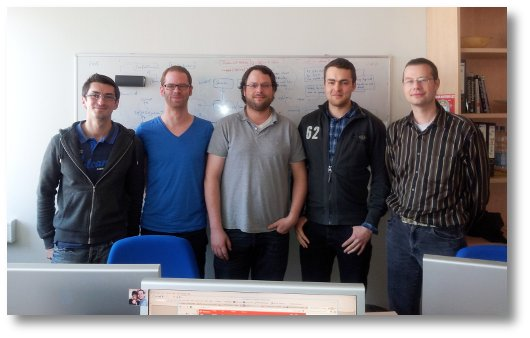
\includegraphics[width=\textwidth]{../rmf-images/2012_03_sprint_team.jpg}
  \caption{The RMF team during a Sprint in April 2012 in Düsseldorf, Germany}
  \label{fig:intro_core_team}
\end{figure}

Many parties were involved in creating RMF we would like to thank the core team that made it possible.

The roots of this project were created by Andreas Graf, Michael Jastram and Nirmal Sasidharan, who joined their various projects together.  Their efforts were financed by the research projects itea Verde and FP7 Deploy.  Together, they brought the project to the Eclipse Foundation, where it has been an active project ever since.  Figure~\ref{fig:intro_core_team} shows four of the five RMF Committers at a joint coding session (missing is Andreas Graf).


